% Auto-generated by analysis/semantic/oncoco/make_hero_tikz.py -- do not edit by hand.
\documentclass[border=1pt,10pt]{standalone}
\usepackage[T1]{fontenc}
\usepackage[scaled=0.92]{helvet}
\renewcommand{\familydefault}{\sfdefault}
\usepackage{sansmath}
\sansmath
\usepackage{tikz}
\usetikzlibrary{arrows.meta,positioning,calc}

\definecolor{cReal}{HTML}{2C6E63}
\definecolor{cRP}{HTML}{4A6E9B}
\definecolor{cLLM}{HTML}{C0503C}
\definecolor{cAcc}{HTML}{7A5EA6}
\definecolor{cMeas}{HTML}{3F4A57}
\definecolor{cInk}{HTML}{1F2328}
\definecolor{cMute}{HTML}{70757D}
\definecolor{cRule}{HTML}{CFD4DA}
\definecolor{cPanel}{HTML}{FBFBFC}
\definecolor{cBand}{HTML}{E5E9EE}

\begin{document}
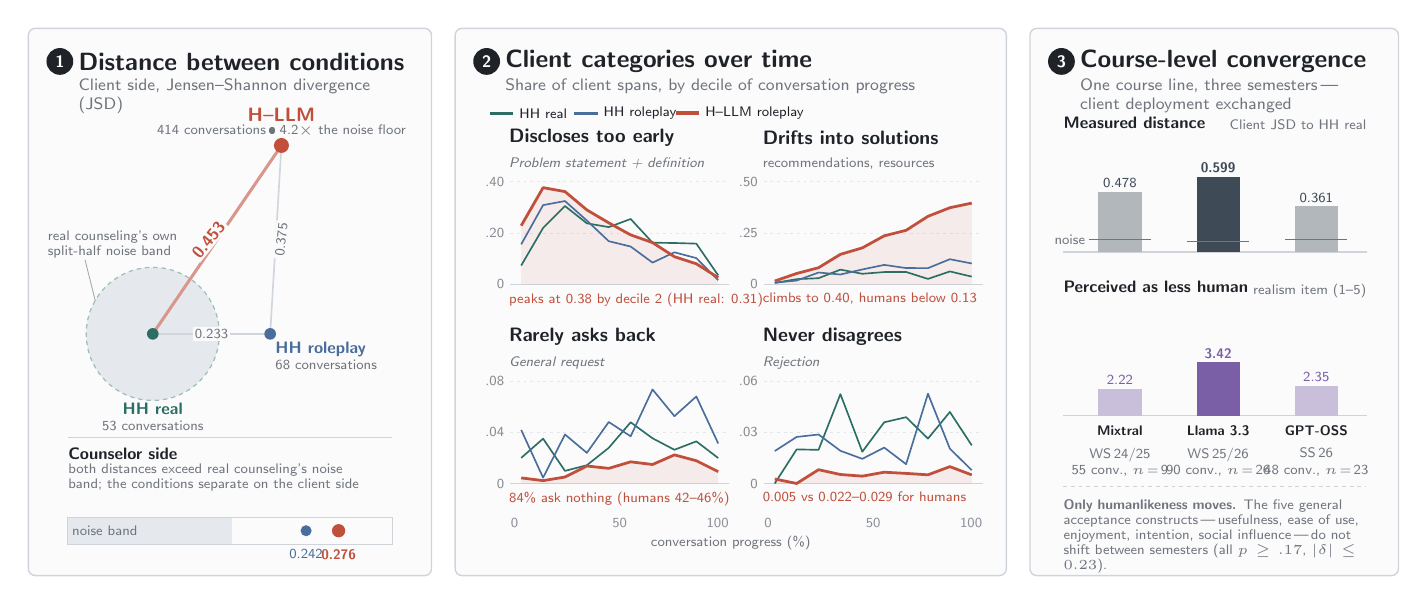
\begin{tikzpicture}[x=1cm,y=1cm]
\path (0,0) rectangle (17.40,6.95);

  \draw[rounded corners=2.5pt, draw=cRule, fill=cPanel, line width=0.5pt]
        (0.00,0) rectangle (5.12,6.95);
  \node[circle, fill=cInk, text=white, inner sep=0pt, minimum size=3.4mm,
        font=\bfseries\fontsize{6}{7}\selectfont] at (0.40,6.53) {1};
  \node[anchor=west, font=\small\bfseries, text=cInk, inner sep=0pt]
        at (0.63,6.53) {Distance between conditions};
  \node[anchor=north west, font=\fontsize{5.6}{6.6}\selectfont, text=cMute, inner sep=0pt,
        align=left, text width=4.17cm] at (0.63,6.31) {Client side, Jensen--Shannon divergence (JSD)};

  \begin{scope}[shift={(1.58,3.07)}]
    \fill[cBand] (0,0) circle (0.845);
    \draw[cReal!45, line width=0.45pt, dash pattern=on 1.6pt off 1.4pt] (0,0) circle (0.845);
    \draw[cRule!95, line width=0.6pt] (0,0) -- (1.491,0);
    \draw[cRule!95, line width=0.6pt] (1.491,0) -- (1.634,2.393);
    \draw[cLLM!60, line width=1.1pt] (0,0) -- (1.634,2.393);
    \node[font=\fontsize{4.7}{5.4}\selectfont, text=cMute, fill=cPanel, inner sep=0.8pt]
         at (0.746,0) {0.233};
    \node[font=\fontsize{4.7}{5.4}\selectfont, text=cMute, fill=cPanel, inner sep=0.8pt, rotate=84]
         at (1.632,1.196) {0.375};
    \node[font=\fontsize{6.4}{7.4}\selectfont\bfseries, text=cLLM, fill=cPanel, inner sep=0.8pt, rotate=51]
         at (0.707,1.196) {0.453};
    \fill[cReal] (0,0) circle (2.1pt);
    \fill[cRP] (1.491,0) circle (2.1pt);
    \fill[cLLM] (1.634,2.393) circle (2.7pt);
    \node[anchor=north, font=\fontsize{6.4}{7.4}\selectfont\bfseries, text=cReal, inner sep=0pt] at (0,-0.875)
         {HH real};
    \node[anchor=north, font=\fontsize{4.7}{5.4}\selectfont, text=cMute, inner sep=0pt] at (0,-1.105)
         {53 conversations};
    \node[anchor=north west, font=\fontsize{6.4}{7.4}\selectfont\bfseries, text=cRP, inner sep=0pt] at (1.551,-0.10)
         {HH roleplay};
    \node[anchor=north west, font=\fontsize{4.7}{5.4}\selectfont, text=cMute, inner sep=0pt] at (1.551,-0.32)
         {68 conversations};
    \node[anchor=south, font=\scriptsize\bfseries, text=cLLM, inner sep=0pt]
         at (1.634,2.693) {H--LLM};
    \node[anchor=south, font=\fontsize{4.7}{5.4}\selectfont, text=cMute, inner sep=0pt]
         at (1.634,2.493)
         {414 conversations\,\textbullet\,4.2$\times$ the noise floor};
  \end{scope}
  \node[anchor=north west, font=\fontsize{4.7}{5.4}\selectfont, text=cMute, align=left, inner sep=0pt]
       at (0.24,4.39) {real counseling's own\\split-half noise band};
  \draw[cMute!65, line width=0.3pt] (0.72,4.01) -- (0.85,3.49);

  \draw[cRule, line width=0.4pt] (0.50,1.75) -- (4.62,1.75);
  \node[anchor=west, font=\fontsize{5.8}{6.8}\selectfont\bfseries, text=cInk, inner sep=0pt] at (0.50,1.55)
       {Counselor side};
  \node[anchor=north west, font=\fontsize{4.7}{5.4}\selectfont, text=cMute, align=left, inner sep=0pt, text width=3.9cm]
       at (0.50,1.43)
       {both distances exceed real counseling's noise band; the conditions separate on the client side};
  \fill[cBand] (0.50,0.40) rectangle (2.592,0.74);
  \draw[cRule, line width=0.4pt] (0.50,0.40) rectangle (4.62,0.74);
  \node[anchor=west, font=\fontsize{4.7}{5.4}\selectfont, text=cMute, inner sep=1.4pt] at (0.50,0.57)
       {noise band};
  \fill[cRP] (3.527,0.57) circle (2.0pt);
  \fill[cLLM] (3.940,0.57) circle (2.4pt);
  \node[anchor=north, font=\fontsize{4.7}{5.4}\selectfont, text=cRP, inner sep=1.8pt] at (3.527,0.40)
       {0.242};
  \node[anchor=north, font=\fontsize{5.2}{6.0}\selectfont\bfseries, text=cLLM, inner sep=1.8pt] at (3.940,0.40)
       {0.276};

  \draw[rounded corners=2.5pt, draw=cRule, fill=cPanel, line width=0.5pt]
        (5.42,0) rectangle (12.42,6.95);
  \node[circle, fill=cInk, text=white, inner sep=0pt, minimum size=3.4mm,
        font=\bfseries\fontsize{6}{7}\selectfont] at (5.82,6.53) {2};
  \node[anchor=west, font=\small\bfseries, text=cInk, inner sep=0pt]
        at (6.05,6.53) {Client categories over time};
  \node[anchor=north west, font=\fontsize{5.6}{6.6}\selectfont, text=cMute, inner sep=0pt,
        align=left, text width=6.05cm] at (6.05,6.31) {Share of client spans, by decile of conversation progress};
  \draw[cReal, line width=0.9pt] (5.86,5.87) -- (6.16,5.87);
  \node[anchor=west, font=\fontsize{4.7}{5.4}\selectfont, text=cInk, inner sep=0pt] at (6.23,5.87) {HH real};
  \draw[cRP, line width=0.9pt] (6.93,5.87) -- (7.23,5.87);
  \node[anchor=west, font=\fontsize{4.7}{5.4}\selectfont, text=cInk, inner sep=0pt] at (7.30,5.87) {HH roleplay};
  \draw[cLLM, line width=1.4pt] (8.22,5.87) -- (8.52,5.87);
  \node[anchor=west, font=\fontsize{4.7}{5.4}\selectfont, text=cInk, inner sep=0pt] at (8.59,5.87) {H--LLM roleplay};

  \begin{scope}[shift={(6.12,3.70)}]
  \draw[cRule, line width=0.4pt] (0,0) -- (2.78,0);
  \draw[cRule!55, line width=0.3pt, dash pattern=on 1pt off 1.4pt] (0,0.650) -- (2.78,0.650);
  \draw[cRule!55, line width=0.3pt, dash pattern=on 1pt off 1.4pt] (0,1.300) -- (2.78,1.300);
  \node[anchor=east, font=\fontsize{4.7}{5.4}\selectfont, text=cMute!85, inner sep=0pt] at (-0.07,0.000) {0};
  \node[anchor=east, font=\fontsize{4.7}{5.4}\selectfont, text=cMute!85, inner sep=0pt] at (-0.07,0.650) {.20};
  \node[anchor=east, font=\fontsize{4.7}{5.4}\selectfont, text=cMute!85, inner sep=0pt] at (-0.07,1.300) {.40};
  \fill[cLLM, opacity=0.09] (0.139,0) -- plot coordinates {(0.139,0.744) (0.417,1.227) (0.695,1.177) (0.973,0.944) (1.251,0.780) (1.529,0.627) (1.807,0.529) (2.085,0.350) (2.363,0.260) (2.641,0.084)} -- (2.641,0) -- cycle;
  \draw[cReal, line width=0.6pt, line join=round] plot coordinates {(0.139,0.238) (0.417,0.715) (0.695,0.993) (0.973,0.774) (1.251,0.726) (1.529,0.829) (1.807,0.528) (2.085,0.524) (2.363,0.516) (2.641,0.113)};
  \draw[cRP, line width=0.6pt, line join=round] plot coordinates {(0.139,0.507) (0.417,1.005) (0.695,1.057) (0.973,0.809) (1.251,0.547) (1.529,0.479) (1.807,0.275) (2.085,0.406) (2.363,0.332) (2.641,0.051)};
  \draw[cLLM, line width=1.0pt, line join=round] plot coordinates {(0.139,0.744) (0.417,1.227) (0.695,1.177) (0.973,0.944) (1.251,0.780) (1.529,0.627) (1.807,0.529) (2.085,0.350) (2.363,0.260) (2.641,0.084)};
  \node[anchor=west, font=\scriptsize\bfseries, text=cInk, inner sep=0pt] at (-0.02,1.86) {Discloses too early};
  \node[anchor=west, font=\fontsize{4.7}{5.4}\selectfont, text=cMute, inner sep=0pt] at (-0.02,1.53) {\textit{Problem statement + definition}};
  \node[anchor=north west, font=\fontsize{5.2}{6.0}\selectfont, text=cLLM, inner sep=0pt] at (-0.02,-0.10) {peaks at 0.38 by decile 2 (HH real: 0.31)};
  \end{scope}

  \begin{scope}[shift={(9.34,3.70)}]
  \draw[cRule, line width=0.4pt] (0,0) -- (2.78,0);
  \draw[cRule!55, line width=0.3pt, dash pattern=on 1pt off 1.4pt] (0,0.650) -- (2.78,0.650);
  \draw[cRule!55, line width=0.3pt, dash pattern=on 1pt off 1.4pt] (0,1.300) -- (2.78,1.300);
  \node[anchor=east, font=\fontsize{4.7}{5.4}\selectfont, text=cMute!85, inner sep=0pt] at (-0.07,0.000) {0};
  \node[anchor=east, font=\fontsize{4.7}{5.4}\selectfont, text=cMute!85, inner sep=0pt] at (-0.07,0.650) {.25};
  \node[anchor=east, font=\fontsize{4.7}{5.4}\selectfont, text=cMute!85, inner sep=0pt] at (-0.07,1.300) {.50};
  \fill[cLLM, opacity=0.09] (0.139,0) -- plot coordinates {(0.139,0.041) (0.417,0.137) (0.695,0.210) (0.973,0.380) (1.251,0.462) (1.529,0.615) (1.807,0.685) (2.085,0.863) (2.363,0.972) (2.641,1.031)} -- (2.641,0) -- cycle;
  \draw[cReal, line width=0.6pt, line join=round] plot coordinates {(0.139,0.017) (0.417,0.065) (0.695,0.077) (0.973,0.186) (1.251,0.133) (1.529,0.155) (1.807,0.156) (2.085,0.068) (2.363,0.163) (2.641,0.097)};
  \draw[cRP, line width=0.6pt, line join=round] plot coordinates {(0.139,0.020) (0.417,0.047) (0.695,0.149) (0.973,0.124) (1.251,0.188) (1.529,0.246) (1.807,0.206) (2.085,0.205) (2.363,0.318) (2.641,0.264)};
  \draw[cLLM, line width=1.0pt, line join=round] plot coordinates {(0.139,0.041) (0.417,0.137) (0.695,0.210) (0.973,0.380) (1.251,0.462) (1.529,0.615) (1.807,0.685) (2.085,0.863) (2.363,0.972) (2.641,1.031)};
  \node[anchor=west, font=\scriptsize\bfseries, text=cInk, inner sep=0pt] at (-0.02,1.86) {Drifts into solutions};
  \node[anchor=west, font=\fontsize{4.7}{5.4}\selectfont, text=cMute, inner sep=0pt] at (-0.02,1.53) {recommendations, resources};
  \node[anchor=north west, font=\fontsize{5.2}{6.0}\selectfont, text=cLLM, inner sep=0pt] at (-0.02,-0.10) {climbs to 0.40, humans below 0.13};
  \end{scope}

  \begin{scope}[shift={(6.12,1.17)}]
  \draw[cRule, line width=0.4pt] (0,0) -- (2.78,0);
  \draw[cRule!55, line width=0.3pt, dash pattern=on 1pt off 1.4pt] (0,0.650) -- (2.78,0.650);
  \draw[cRule!55, line width=0.3pt, dash pattern=on 1pt off 1.4pt] (0,1.300) -- (2.78,1.300);
  \node[anchor=east, font=\fontsize{4.7}{5.4}\selectfont, text=cMute!85, inner sep=0pt] at (-0.07,0.000) {0};
  \node[anchor=east, font=\fontsize{4.7}{5.4}\selectfont, text=cMute!85, inner sep=0pt] at (-0.07,0.650) {.04};
  \node[anchor=east, font=\fontsize{4.7}{5.4}\selectfont, text=cMute!85, inner sep=0pt] at (-0.07,1.300) {.08};
  \fill[cLLM, opacity=0.09] (0.139,0) -- plot coordinates {(0.139,0.071) (0.417,0.036) (0.695,0.082) (0.973,0.222) (1.251,0.192) (1.529,0.275) (1.807,0.241) (2.085,0.363) (2.363,0.289) (2.641,0.150)} -- (2.641,0) -- cycle;
  \draw[cReal, line width=0.6pt, line join=round] plot coordinates {(0.139,0.325) (0.417,0.569) (0.695,0.160) (0.973,0.232) (1.251,0.453) (1.529,0.777) (1.807,0.574) (2.085,0.428) (2.363,0.535) (2.641,0.323)};
  \draw[cRP, line width=0.6pt, line join=round] plot coordinates {(0.139,0.680) (0.417,0.074) (0.695,0.622) (0.973,0.389) (1.251,0.781) (1.529,0.599) (1.807,1.194) (2.085,0.855) (2.363,1.105) (2.641,0.508)};
  \draw[cLLM, line width=1.0pt, line join=round] plot coordinates {(0.139,0.071) (0.417,0.036) (0.695,0.082) (0.973,0.222) (1.251,0.192) (1.529,0.275) (1.807,0.241) (2.085,0.363) (2.363,0.289) (2.641,0.150)};
  \node[anchor=west, font=\scriptsize\bfseries, text=cInk, inner sep=0pt] at (-0.02,1.86) {Rarely asks back};
  \node[anchor=west, font=\fontsize{4.7}{5.4}\selectfont, text=cMute, inner sep=0pt] at (-0.02,1.53) {\textit{General request}};
  \node[anchor=north west, font=\fontsize{5.2}{6.0}\selectfont, text=cLLM, inner sep=0pt] at (-0.02,-0.10) {84\% ask nothing (humans 42--46\%)};
  \node[anchor=north west, font=\fontsize{4.7}{5.4}\selectfont, text=cMute!80, inner sep=0pt] at (0.000,-0.44) {0};
  \node[anchor=north, font=\fontsize{4.7}{5.4}\selectfont, text=cMute!80, inner sep=0pt] at (1.390,-0.44) {50};
  \node[anchor=north east, font=\fontsize{4.7}{5.4}\selectfont, text=cMute!80, inner sep=0pt] at (2.780,-0.44) {100};
  \end{scope}

  \begin{scope}[shift={(9.34,1.17)}]
  \draw[cRule, line width=0.4pt] (0,0) -- (2.78,0);
  \draw[cRule!55, line width=0.3pt, dash pattern=on 1pt off 1.4pt] (0,0.650) -- (2.78,0.650);
  \draw[cRule!55, line width=0.3pt, dash pattern=on 1pt off 1.4pt] (0,1.300) -- (2.78,1.300);
  \node[anchor=east, font=\fontsize{4.7}{5.4}\selectfont, text=cMute!85, inner sep=0pt] at (-0.07,0.000) {0};
  \node[anchor=east, font=\fontsize{4.7}{5.4}\selectfont, text=cMute!85, inner sep=0pt] at (-0.07,0.650) {.03};
  \node[anchor=east, font=\fontsize{4.7}{5.4}\selectfont, text=cMute!85, inner sep=0pt] at (-0.07,1.300) {.06};
  \fill[cLLM, opacity=0.09] (0.139,0) -- plot coordinates {(0.139,0.057) (0.417,0.000) (0.695,0.175) (0.973,0.114) (1.251,0.093) (1.529,0.143) (1.807,0.128) (2.085,0.110) (2.363,0.214) (2.641,0.109)} -- (2.641,0) -- cycle;
  \draw[cReal, line width=0.6pt, line join=round] plot coordinates {(0.139,0.000) (0.417,0.433) (0.695,0.427) (0.973,1.135) (1.251,0.403) (1.529,0.777) (1.807,0.842) (2.085,0.570) (2.363,0.908) (2.641,0.484)};
  \draw[cRP, line width=0.6pt, line join=round] plot coordinates {(0.139,0.412) (0.417,0.591) (0.695,0.622) (0.973,0.415) (1.251,0.313) (1.529,0.456) (1.807,0.245) (2.085,1.140) (2.363,0.442) (2.641,0.169)};
  \draw[cLLM, line width=1.0pt, line join=round] plot coordinates {(0.139,0.057) (0.417,0.000) (0.695,0.175) (0.973,0.114) (1.251,0.093) (1.529,0.143) (1.807,0.128) (2.085,0.110) (2.363,0.214) (2.641,0.109)};
  \node[anchor=west, font=\scriptsize\bfseries, text=cInk, inner sep=0pt] at (-0.02,1.86) {Never disagrees};
  \node[anchor=west, font=\fontsize{4.7}{5.4}\selectfont, text=cMute, inner sep=0pt] at (-0.02,1.53) {\textit{Rejection}};
  \node[anchor=north west, font=\fontsize{5.2}{6.0}\selectfont, text=cLLM, inner sep=0pt] at (-0.02,-0.10) {0.005 vs 0.022--0.029 for humans};
  \node[anchor=north west, font=\fontsize{4.7}{5.4}\selectfont, text=cMute!80, inner sep=0pt] at (0.000,-0.44) {0};
  \node[anchor=north, font=\fontsize{4.7}{5.4}\selectfont, text=cMute!80, inner sep=0pt] at (1.390,-0.44) {50};
  \node[anchor=north east, font=\fontsize{4.7}{5.4}\selectfont, text=cMute!80, inner sep=0pt] at (2.780,-0.44) {100};
  \end{scope}
  \node[anchor=north, font=\fontsize{4.7}{5.4}\selectfont, text=cMute, inner sep=0pt]
       at (8.92,0.51) {conversation progress (\%)};

  \draw[rounded corners=2.5pt, draw=cRule, fill=cPanel, line width=0.5pt]
        (12.72,0) rectangle (17.40,6.95);
  \node[circle, fill=cInk, text=white, inner sep=0pt, minimum size=3.4mm,
        font=\bfseries\fontsize{6}{7}\selectfont] at (13.12,6.53) {3};
  \node[anchor=west, font=\small\bfseries, text=cInk, inner sep=0pt]
        at (13.35,6.53) {Course-level convergence};
  \node[anchor=north west, font=\fontsize{5.6}{6.6}\selectfont, text=cMute, inner sep=0pt,
        align=left, text width=3.73cm] at (13.35,6.31) {One course line, three semesters\,---\,client deployment exchanged};
  \node[anchor=north west, font=\fontsize{5.8}{6.8}\selectfont\bfseries, text=cInk, inner sep=0pt]
       at (13.14,5.83) {Measured distance};
  \node[anchor=north east, font=\fontsize{4.7}{5.4}\selectfont, text=cMute, inner sep=0pt]
       at (17.00,5.79) {Client JSD to HH real};
  \draw[cRule, line width=0.4pt] (13.14,4.11) -- (17.00,4.11);
  \fill[cMeas!40] (13.589,4.110) rectangle (14.138,4.875);
  \node[anchor=south, font=\fontsize{5.2}{6.0}\selectfont, text=cMeas, inner sep=1.3pt] at (13.863,4.875) {0.478};
  \fill[cMeas] (14.836,4.110) rectangle (15.384,5.068);
  \node[anchor=south, font=\fontsize{5.2}{6.0}\selectfont\bfseries, text=cMeas, inner sep=1.3pt] at (15.110,5.068) {0.599};
  \fill[cMeas!40] (16.082,4.110) rectangle (16.631,4.688);
  \node[anchor=south, font=\fontsize{5.2}{6.0}\selectfont, text=cMeas, inner sep=1.3pt] at (16.357,4.688) {0.361};
  \draw[cMute, line width=0.5pt] (13.468,4.265) -- (14.258,4.265);
  \draw[cMute, line width=0.5pt] (14.715,4.246) -- (15.505,4.246);
  \draw[cMute, line width=0.5pt] (15.962,4.268) -- (16.752,4.268);
  \node[anchor=east, font=\fontsize{4.7}{5.4}\selectfont, text=cMute, inner sep=1.2pt] at (13.47,4.27) {noise};
  \node[anchor=north west, font=\fontsize{5.8}{6.8}\selectfont\bfseries, text=cInk, inner sep=0pt]
       at (13.14,3.75) {Perceived as \emph{less} human};
  \node[anchor=north east, font=\fontsize{4.7}{5.4}\selectfont, text=cMute, inner sep=0pt]
       at (17.00,3.71) {realism item (1--5)};
  \draw[cRule, line width=0.4pt] (13.14,2.03) -- (17.00,2.03);
  \fill[cAcc!40] (13.589,2.030) rectangle (14.138,2.372);
  \node[anchor=south, font=\fontsize{5.2}{6.0}\selectfont, text=cAcc, inner sep=1.3pt] at (13.863,2.372) {2.22};
  \fill[cAcc] (14.836,2.030) rectangle (15.384,2.708);
  \node[anchor=south, font=\fontsize{5.2}{6.0}\selectfont\bfseries, text=cAcc, inner sep=1.3pt] at (15.110,2.708) {3.42};
  \fill[cAcc!40] (16.082,2.030) rectangle (16.631,2.408);
  \node[anchor=south, font=\fontsize{5.2}{6.0}\selectfont, text=cAcc, inner sep=1.3pt] at (16.357,2.408) {2.35};
  \node[anchor=north, font=\fontsize{5.2}{6.0}\selectfont\bfseries, text=cInk, inner sep=1.3pt]
       at (13.863,1.95) {Mixtral};
  \node[anchor=north, font=\fontsize{4.7}{5.4}\selectfont, text=cMute, inner sep=1.1pt]
       at (13.863,1.67) {WS\,24/25};
  \node[anchor=north, font=\fontsize{4.7}{5.4}\selectfont, text=cMute, inner sep=1.1pt]
       at (13.863,1.45) {55 conv., $n$\,=\,9};
  \node[anchor=north, font=\fontsize{5.2}{6.0}\selectfont\bfseries, text=cInk, inner sep=1.3pt]
       at (15.110,1.95) {Llama 3.3};
  \node[anchor=north, font=\fontsize{4.7}{5.4}\selectfont, text=cMute, inner sep=1.1pt]
       at (15.110,1.67) {WS\,25/26};
  \node[anchor=north, font=\fontsize{4.7}{5.4}\selectfont, text=cMute, inner sep=1.1pt]
       at (15.110,1.45) {90 conv., $n$\,=\,26};
  \node[anchor=north, font=\fontsize{5.2}{6.0}\selectfont\bfseries, text=cInk, inner sep=1.3pt]
       at (16.357,1.95) {GPT-OSS};
  \node[anchor=north, font=\fontsize{4.7}{5.4}\selectfont, text=cMute, inner sep=1.1pt]
       at (16.357,1.67) {SS\,26};
  \node[anchor=north, font=\fontsize{4.7}{5.4}\selectfont, text=cMute, inner sep=1.1pt]
       at (16.357,1.45) {48 conv., $n$\,=\,23};

  \draw[cRule, line width=0.4pt, dash pattern=on 1.4pt off 1.4pt]
       (13.14,1.13) -- (16.98,1.13);
  \node[anchor=north west, font=\fontsize{4.7}{5.4}\selectfont, text=cMute, align=left, inner sep=0pt, text width=3.84cm]
       at (13.14,0.97) {\textbf{Only humanlikeness moves.} The five general acceptance
        constructs\,---\,usefulness, ease of use, enjoyment, intention, social influence\,---\,do
        not shift between semesters (all $p\geq.17$, $|\delta|\leq0.23$).};
\end{tikzpicture}
\end{document}
